\section{Home Page}
The home page is how the website appear to users, so it has to give a clear
idea about the content of internal pages. Moreover, it has to provide all
the necessary information to the user in a fast and clear way.\\
Before analyzing it, we define how the home page's structure is composed.

\subsection{Structure}
Here there is a presentation about the home page structure.\\
After entering in the website (figure \ref{home-page-no-scroll}), we can
recognize some elements such as:
\begin{itemize}
    \item internal advertising banner;
    \item banner for contacts, social and sign in button;
    \item logo;
    \item navbar with links for other sections of the website;
    \item search bar;
    \item favourites, product comparison and bucket buttons;
    \item big image (more information in section );
\end{itemize}
\newpage
\vspace*{\fill}
\begin{figure}[!h] 
    \centering 
    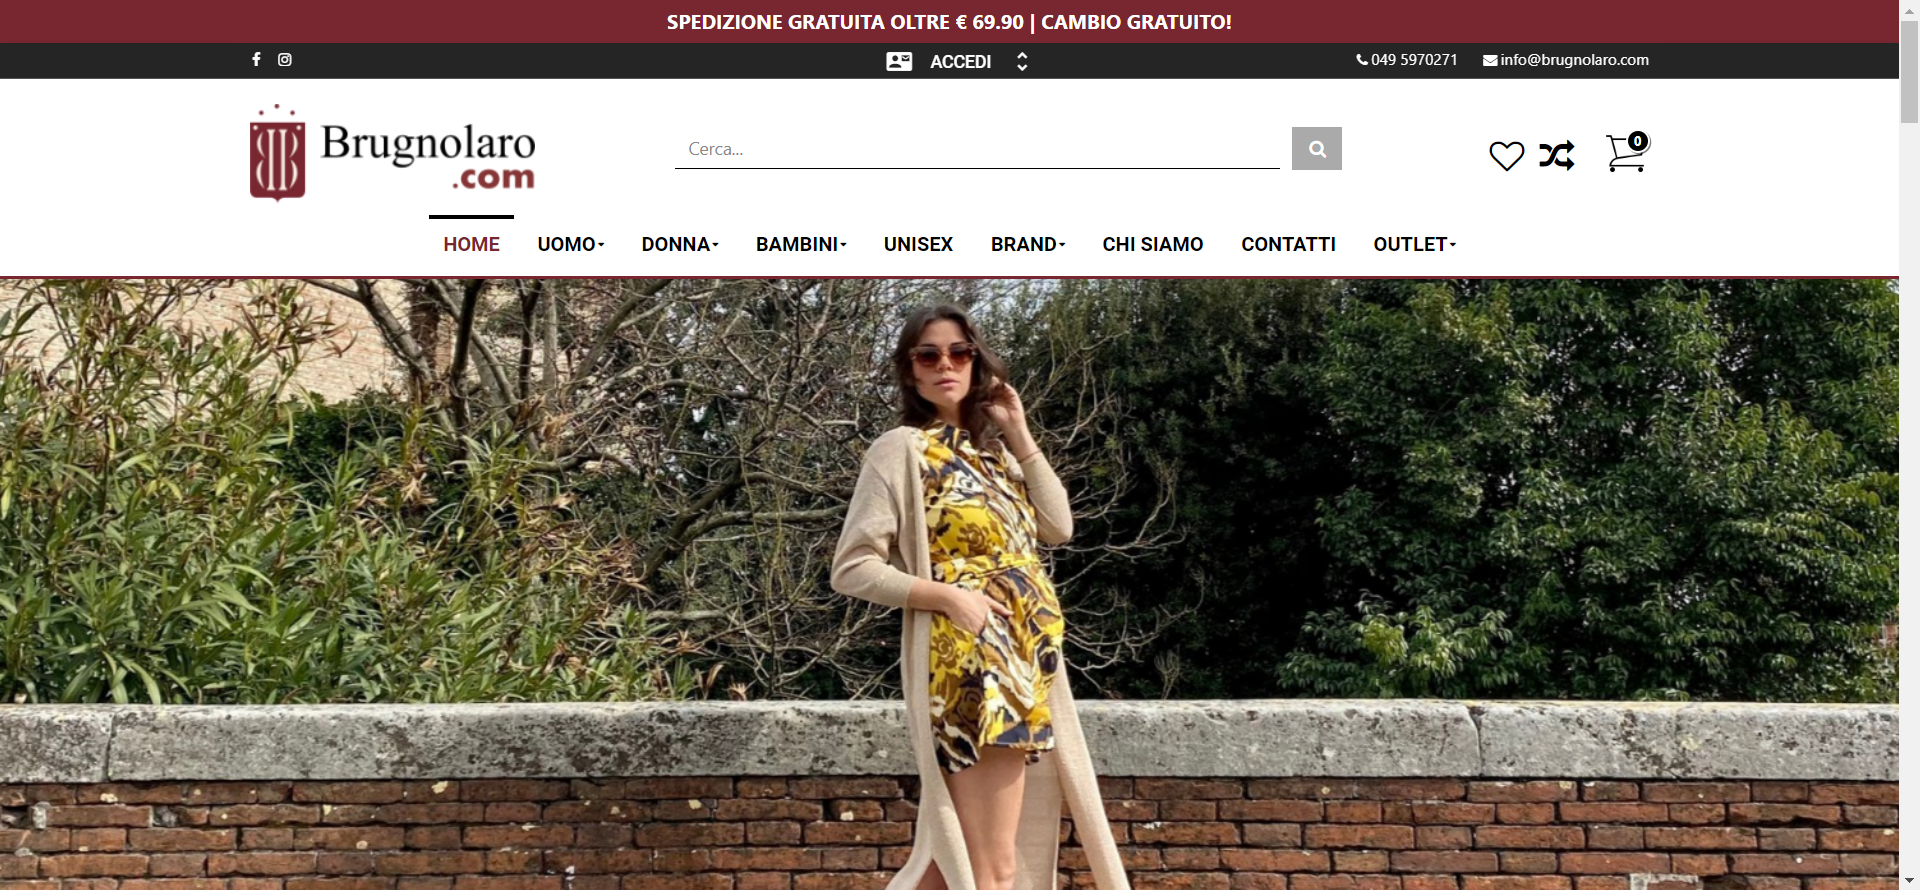
\includegraphics[scale = 0.29]{images/hp_scroll0.png} 
    \caption{Home page (first presentation)}
    \label{home-page-no-scroll}
\end{figure}
\vspace*{\fill}
\vspace*{\fill}
Going down using the scroll, there are some suggestions for the
e-commerce sections (figure \ref{home-page-scroll-1}).
\vspace*{\fill}
\vspace*{\fill}
\begin{figure}[!h] 
    \centering 
    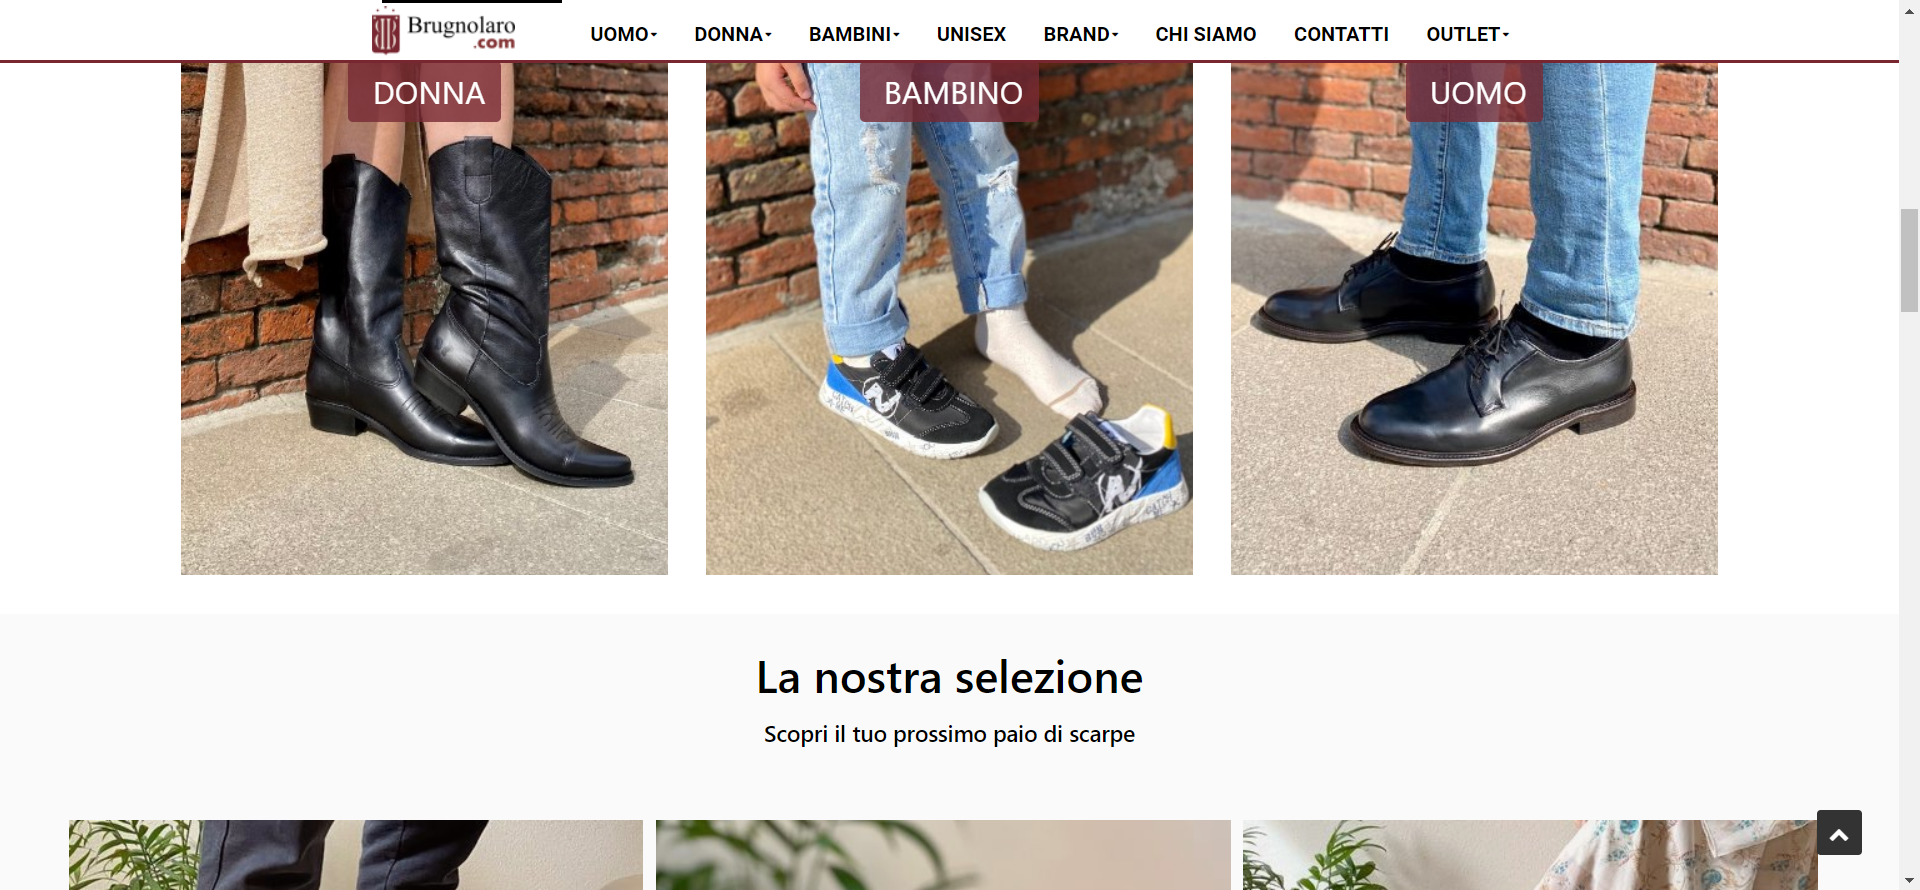
\includegraphics[scale = 0.29]{images/hp_scroll1.png} 
    \caption{Home page (e-commerce selection)}
    \label{home-page-scroll-1}
\end{figure}
\vspace*{\fill}
\newpage
Then there are some informations about customer experiences and
brands the company sells (figure \ref{home-page-scroll-2}).
\begin{figure}[!h] 
    \centering 
    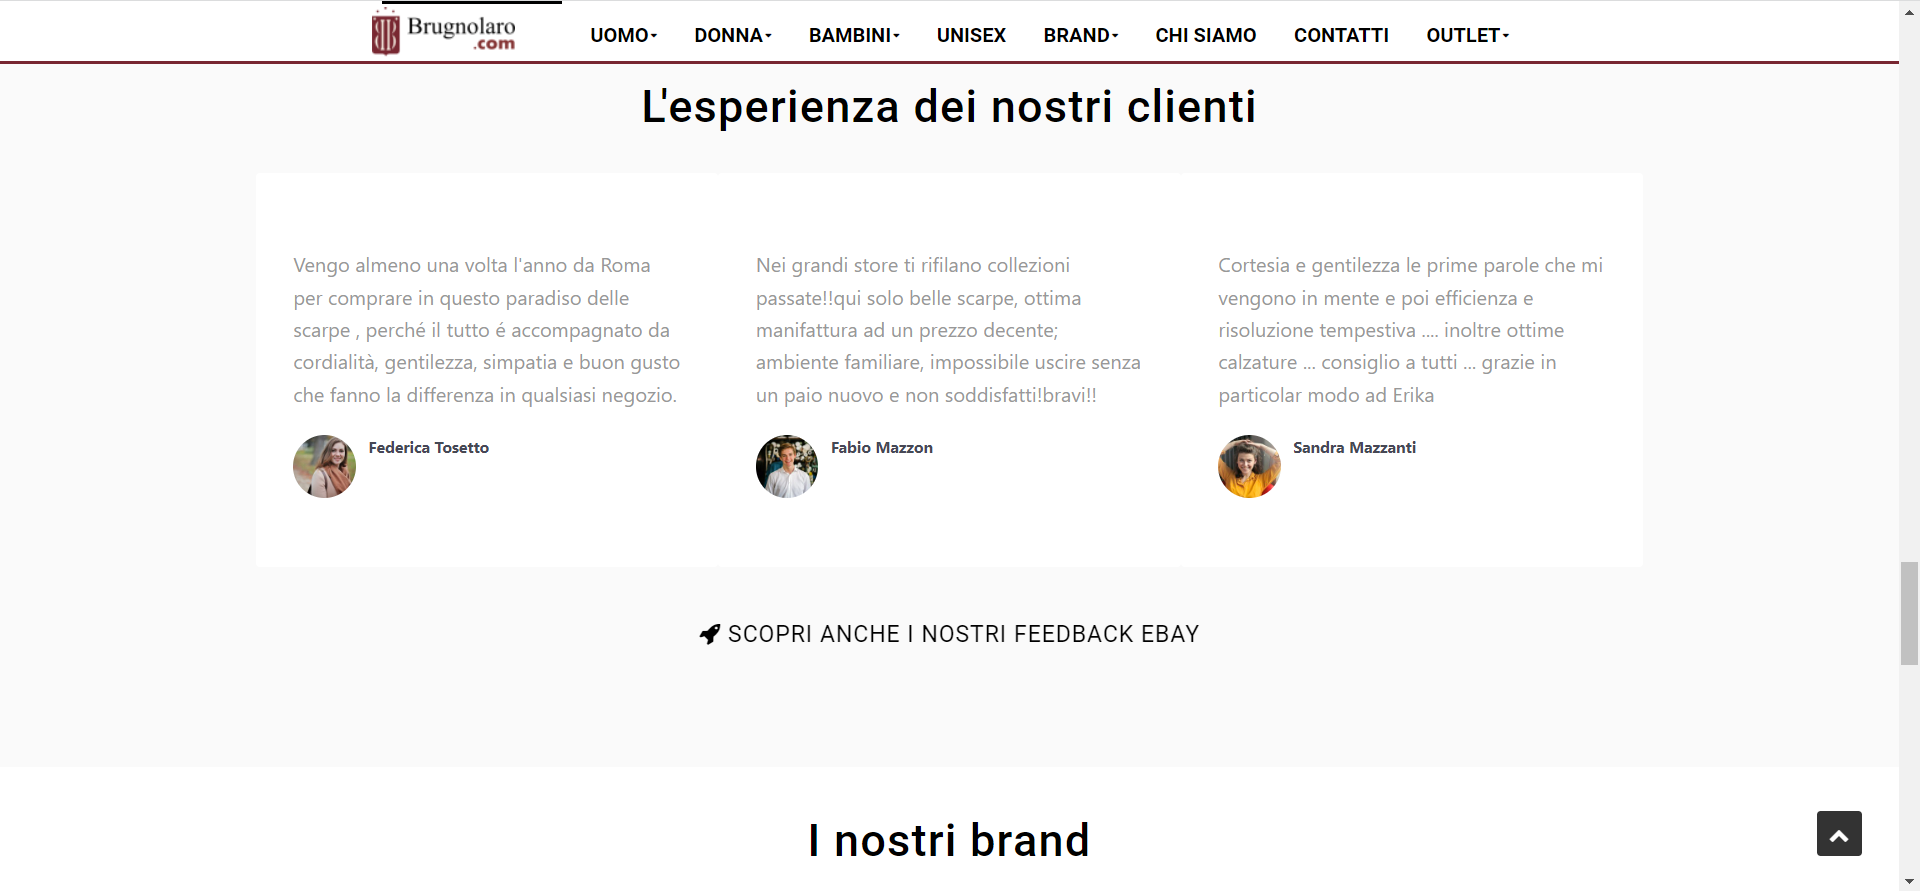
\includegraphics[scale = 0.29]{images/hp_scroll2.png} 
    \caption{Home page (customers experience and brands)}
    \label{home-page-scroll-2}
\end{figure}
\newline
Finally, there is a footer at the bottom of the page which contains
the possibility of subscription to the newsletter website and many other
informations (figure \ref{home-page-scroll-3}).
\begin{figure}[!h] 
    \centering 
    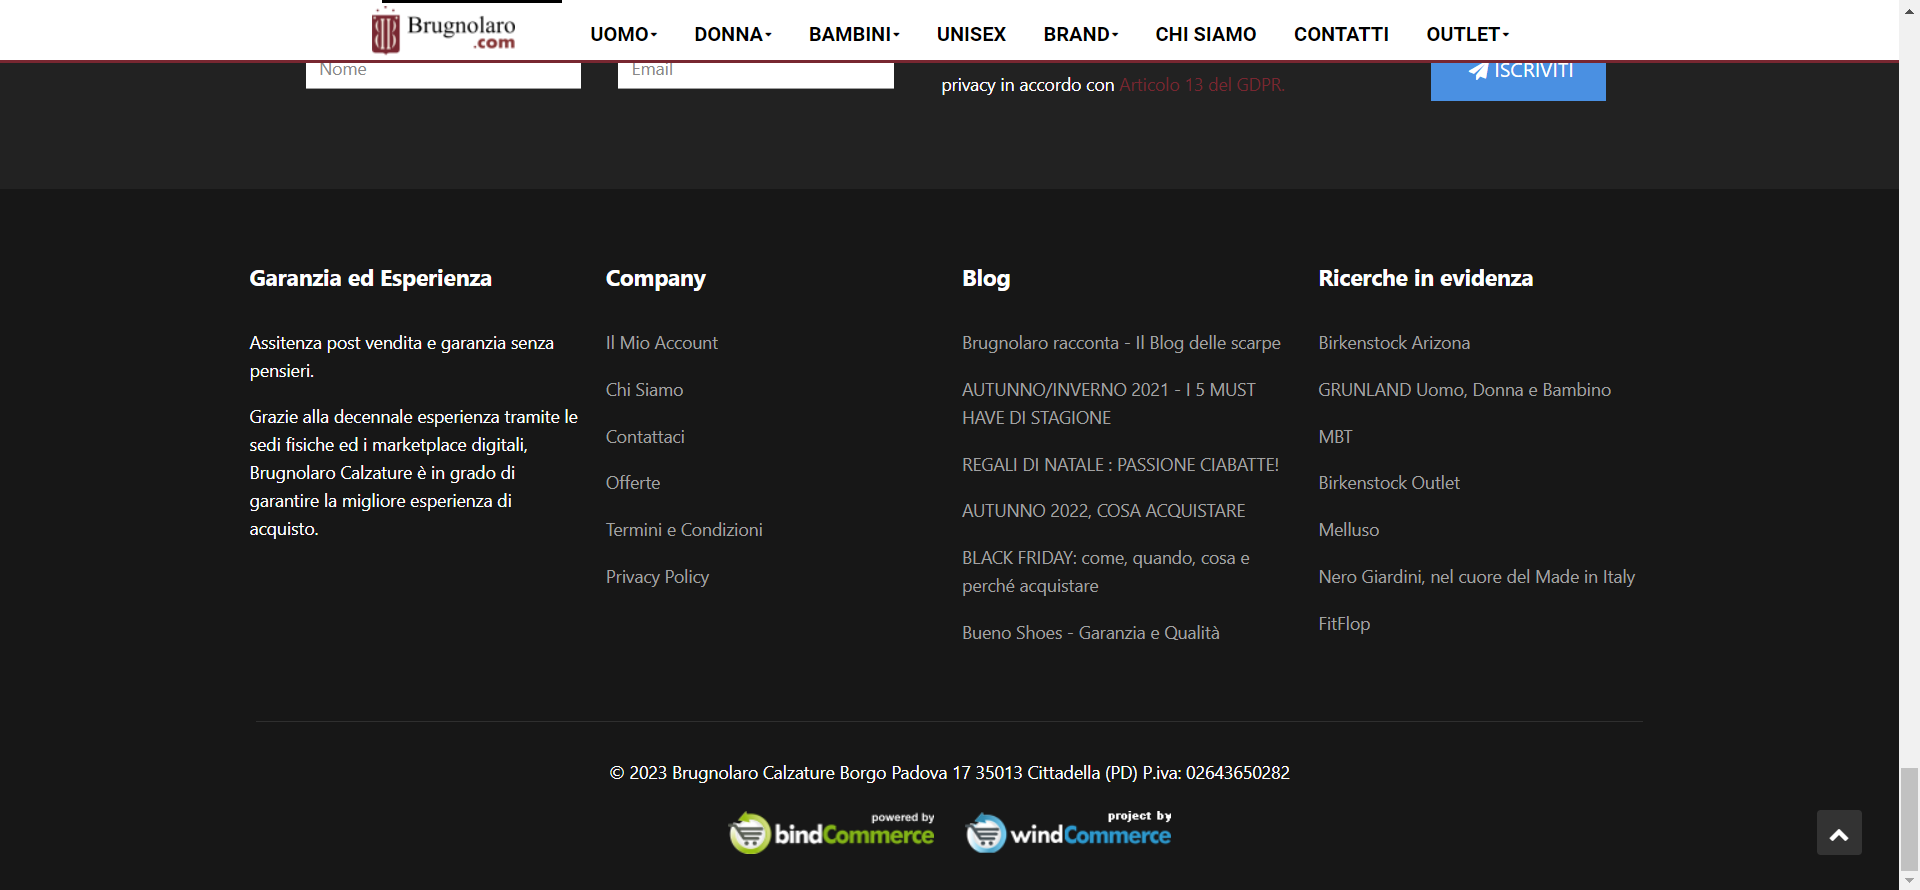
\includegraphics[scale = 0.29]{images/hp_scroll3.png} 
    \caption{Home page (footer)}
    \label{home-page-scroll-3}
\end{figure}
\subsection{Informative axes}
During the design of a webpage, it is important to answer first
to what in journalism is called the 6 \textit{W} which are:
\begin{itemize}
    \item Where?
    \item Who?
    \item Why?
    \item What?
    \item When?
    \item How?
\end{itemize}
This can enable the possibility for people to collect the main informations which are
essential for their permanence in the website.
\subsubsection{WHERE did the user arrive?}
A webpage should allow to the users to know about their relative position
in the website. If the "\textit{where}" axis is not there,
the user may feel lost, which is a sensation that may make the user angry.\\

When the user enters directly in the home page for the first time (fig. \ref{home-page-no-scroll}), he will see a
complete menu, which contains all the destinations available. That is
really good. In fact the user can find easily his way for what he is searching for.\\
There is no breadcrumbs in the home page. It should always appear in order
to make the users able to understand where they are placed in the website, but in this
particular case it could be acceptable.

\subsubsection{WHO is behind the website?}
A webpage should give the information about the website's owner, so "\textit{who}" is
behind the website.\\

There is the Brugnolaro's logo on the top-left corner, which is really good to immediately get the
identity of the website's owner. Maybe a little critic could be about that the logo's position
is a little decentered from the top-left's magic spot, but still it doesn't care. It is clear
also that the logo would work only if the user already knows the company and what they do.\\
Another place where the user can find information about the owner is on the footer (scrolling
so much!). Here he can see more details such as "\textit{Chi siamo}", "\textit{Contattaci}" or
the copyright notification with the sponsor which has been used to construct the website.
(figure \ref{home-page-scroll-3-circle})

\begin{figure}[!h] 
    \centering 
    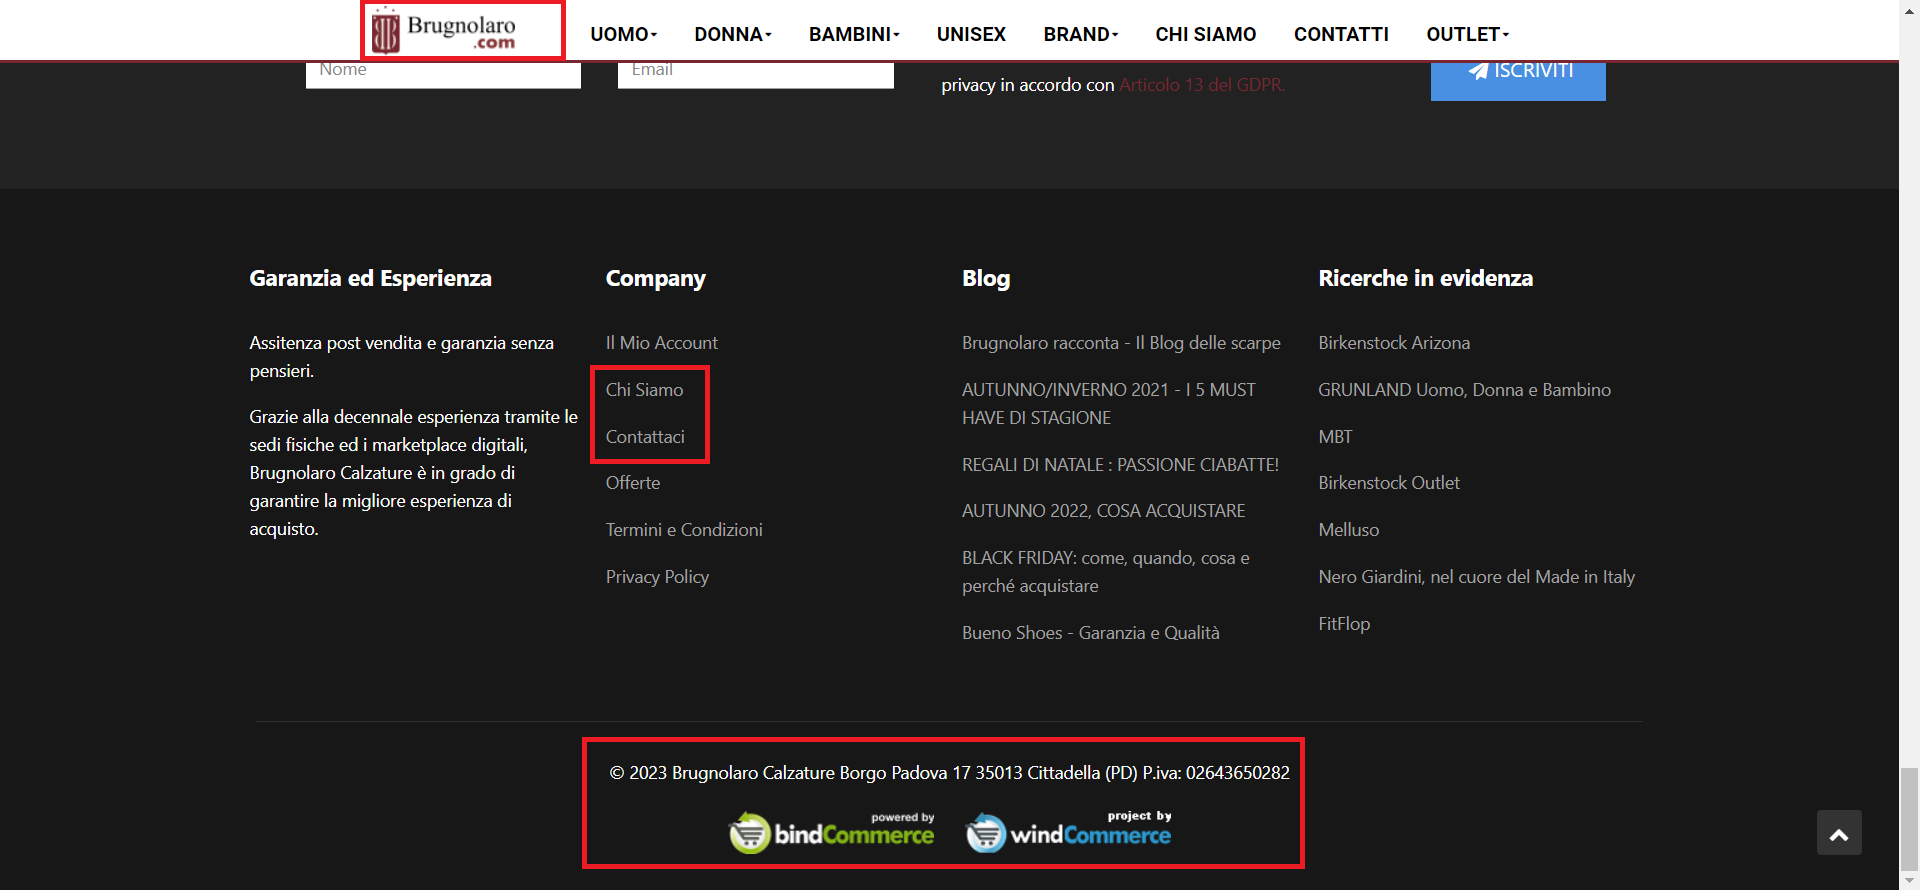
\includegraphics[scale = 0.29]{images/hp_scroll3_circle.png} 
    \caption{Home page (footer who)}
    \label{home-page-scroll-3-circle}
\end{figure}

\subsubsection{WHY should the user stay?}
A webpage page should provide motivations to users to persuade them to stay and navigate within
the website.\\

Watching the homepage with no scroll, there is no indication about any reason to stay, but, if we scroll a little bit,
there is a section dedicated to customers' reviews. This could be very useful because the owner
expose himself to the judgment of customers without any fear (giving also the possibility to
the user to see eBay's reviews) (figure \ref{home-page-scroll-2}).\\
There are also the brief description of some advantages given by the company to the customers
and could play an important role too (figure \ref{home-page-why}).
\begin{figure}[!h] 
    \centering 
    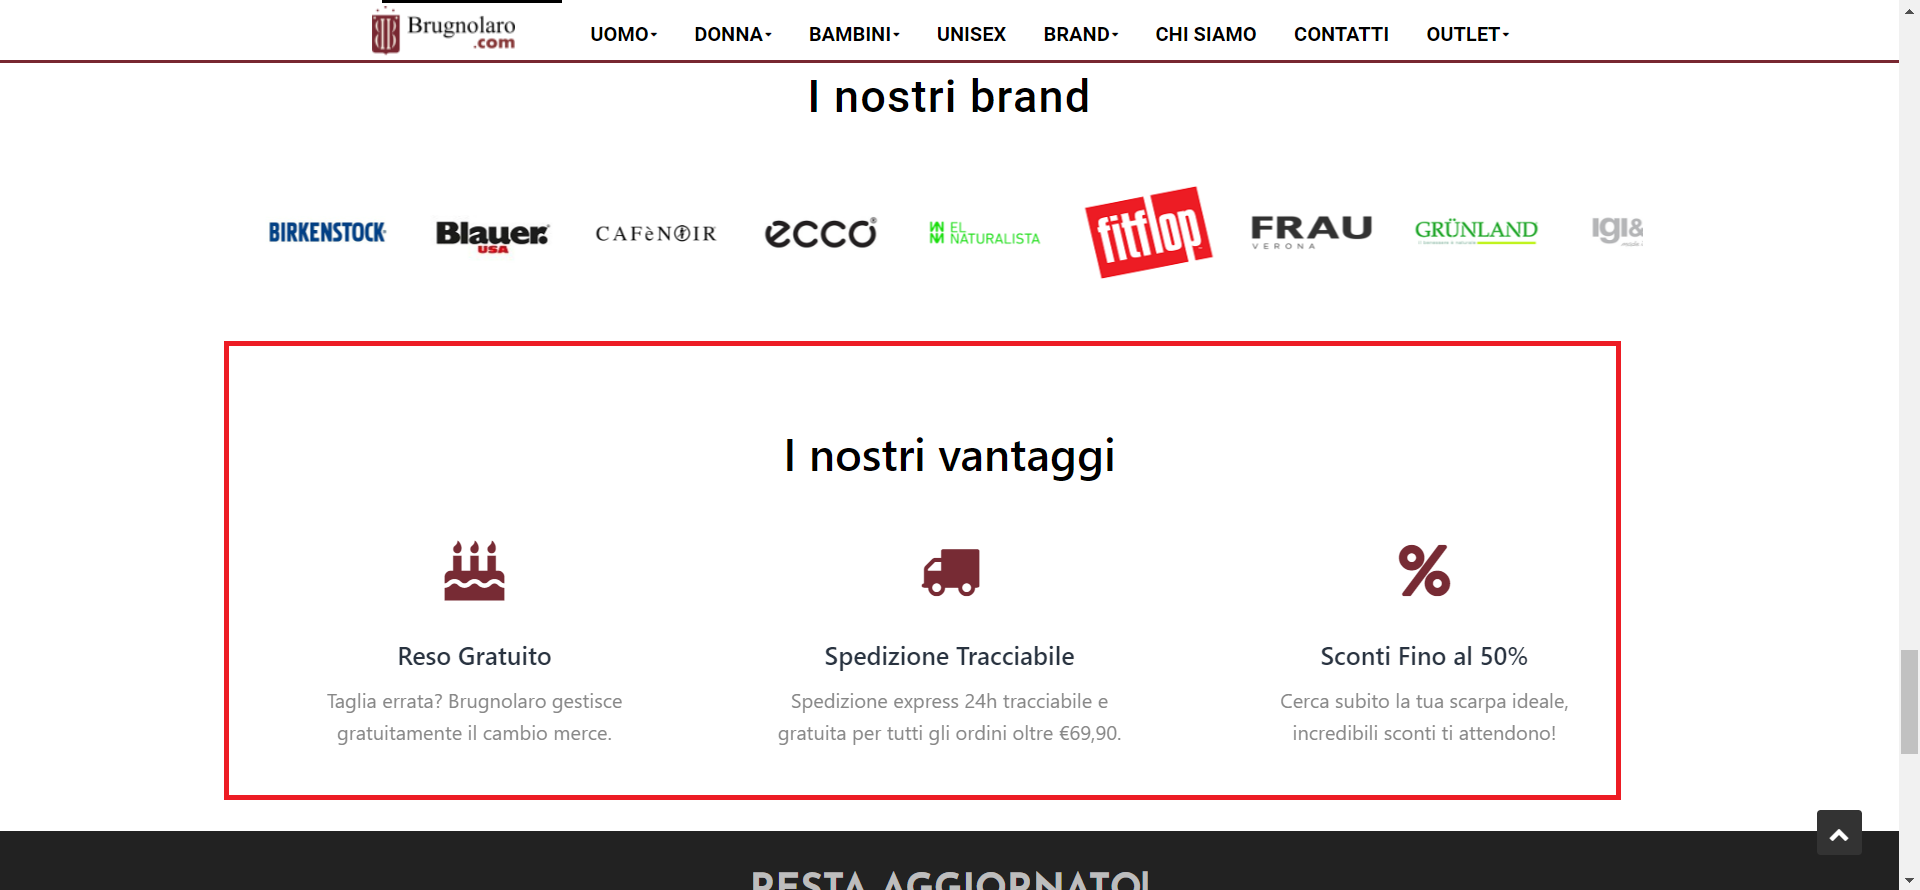
\includegraphics[scale = 0.29]{images/why.png} 
    \caption{Home page (why)}
    \label{home-page-why}
\end{figure}
\newline
I think that this content which has the goal to convince users to stay in the website should be
moved up in order not to force the user to make so much scroll which creates a lot of computational effort.

\subsubsection{WHAT choices does the user have?}\label{what}
A webpage should give the users access to all the possible
destinations of the website.\\
Here there is the menu (more infomration in section ) which basically provides all macro searches
for a particular kind of articles. This speed up the search of the user to a specific product and
it is considered a good thing. There is also the expansion of the menu in which the user can choose
a more specific category and this provides a very good pace in terms of navigation
(figure \ref{home-page-what}).\\

Finally the presence of relevant searches in the footer can also be a good idea for
speeding up main researches (figure \ref{home-page-scroll-3})
\begin{figure}[!h] 
    \centering 
    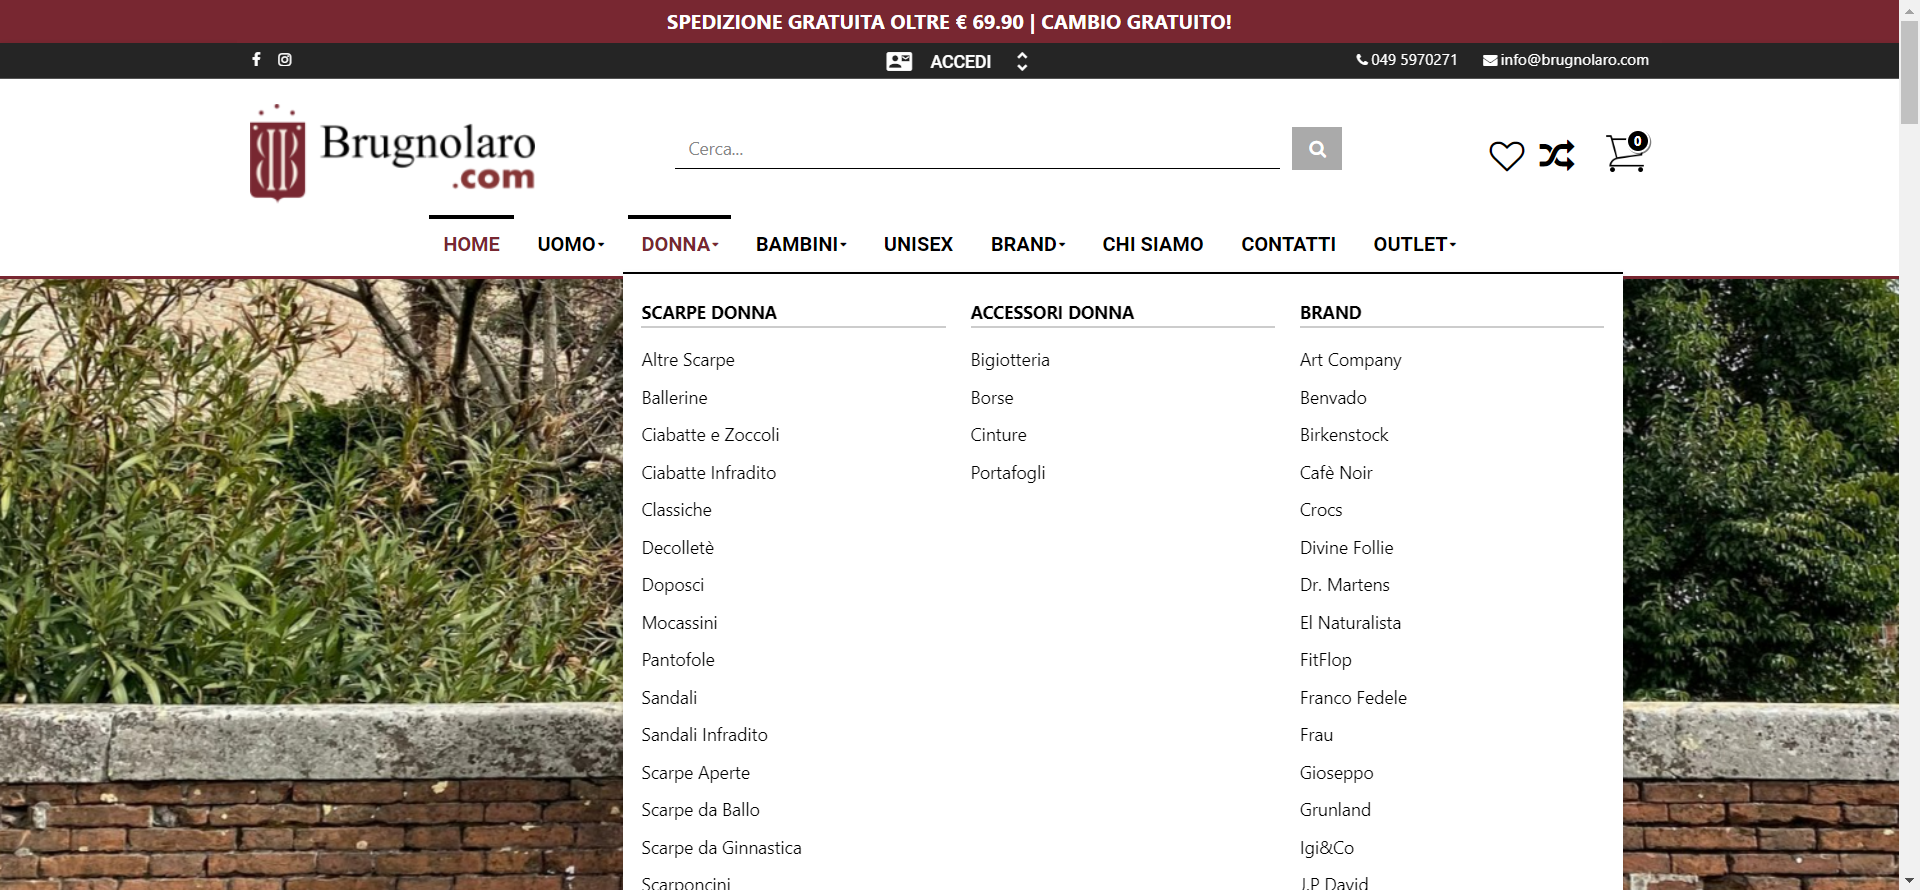
\includegraphics[scale = 0.29]{images/what_menu.png} 
    \caption{Home page (what)}
    \label{home-page-what}
\end{figure}
\newpage
\subsubsection{WHEN (latest news)}
A webpage should provide to the users all the latest news regarding the products and the company.\\

There are two things tha suggest something similar, even if is not intuitive and the user
could not be able to find it in an easy way.
The first one is the blog section in the footer which contains links for blog articles about
what is going on in the company and which are the latest discount and product arrivals.
The last one is about the newsletter with 5\% of discount if user subscribe with his mail.
\begin{figure}[!h] 
    \centering 
    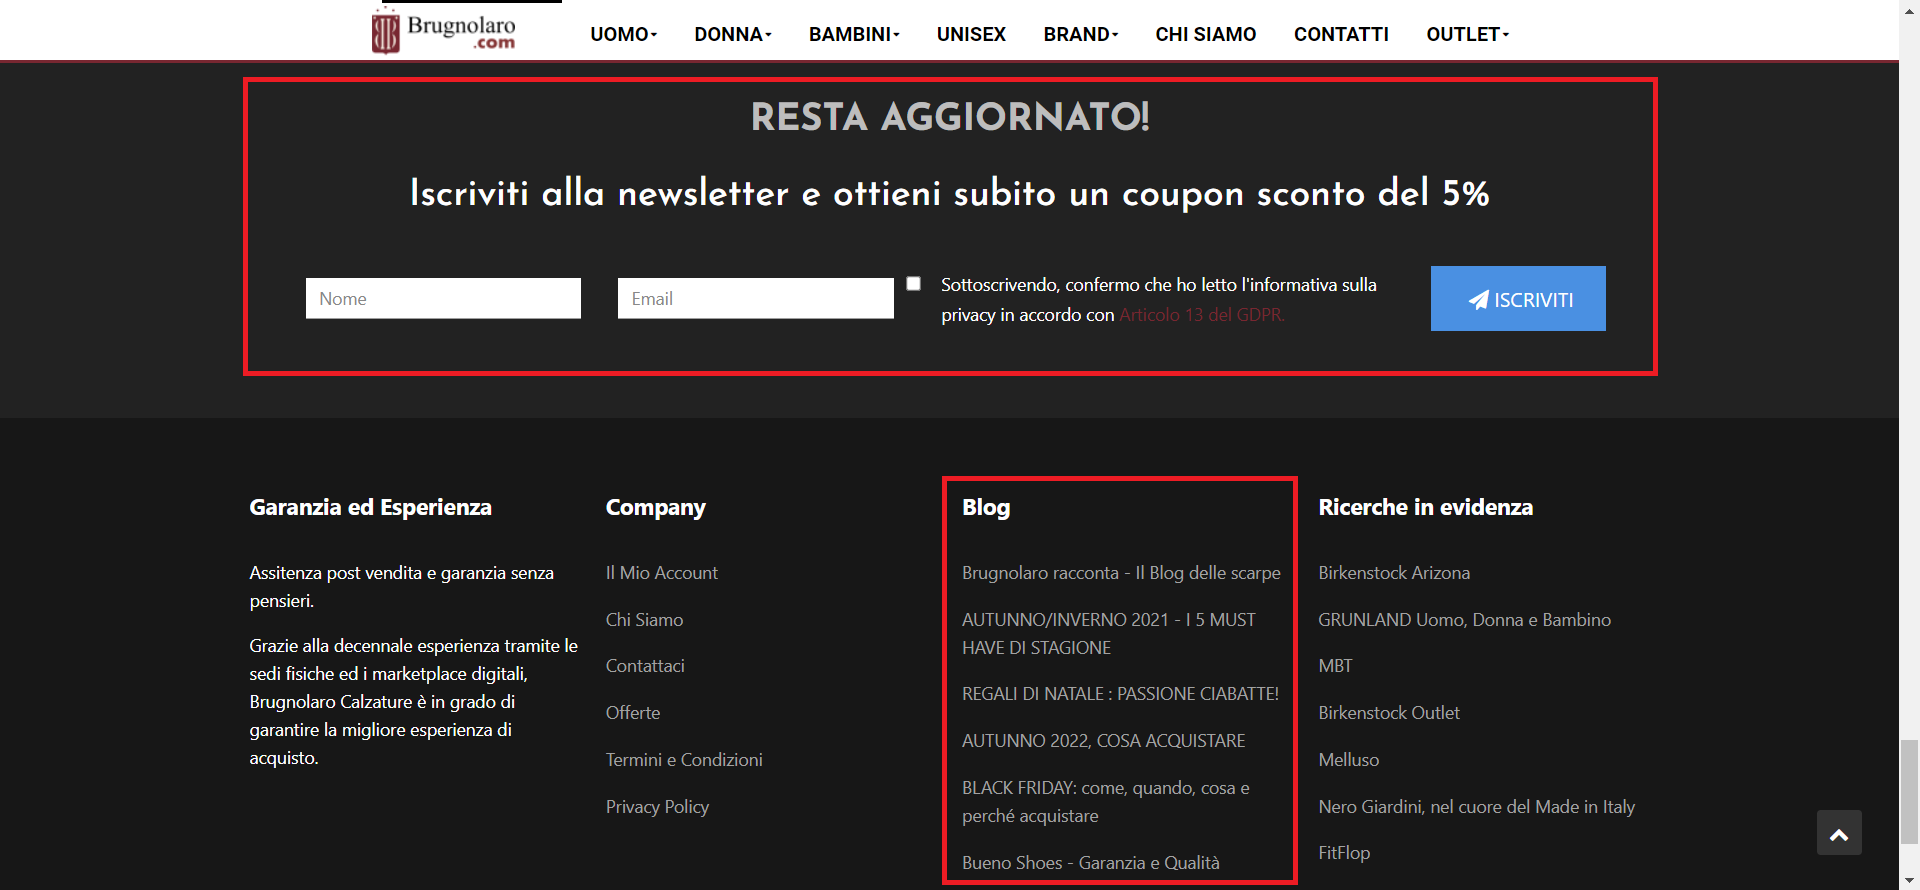
\includegraphics[scale = 0.29]{images/when.png} 
    \caption{Home page (when)}
    \label{home-page-when}
\end{figure}
\newline
The blog is good because it allows to save some space in the page (and scrolling too!) and
it connects directly to the links for the latest news.
The newsletter could be useful for keeping the user aware about news about the company which
are basically what it is written in the blog and it attracts users for the discount, but it has
as drawback the fact that users have to give some data for subscription (which is not desirable).

\subsubsection{HOW to arrive where the user wants?}
A website should offer the possibility to the users to access
and collect information in a fast and smart way.

There is a search bar which very appreciated by the users.\\
Again the menu contains all macro searches and then more precise ones. (see section §\ref{what})

\subsection{Navigation}
The website is not handling the "lost in navigation problem" in an excellent way.
It is true that the menu is shown in both home and internal pages which makes
the user feel more comfortable, but the breadcrumbs are not available.\\

Regarding the way 
the user can understand visited or not visited links, the website is not doing a good job.
In fact there is not any difference
between the colors of visited and not visited links. That is a bad choice because the user has to
be able to remember already visited places. thus the navigation will be heavier because users can forget
pages that they have already visited. Moreover if they visit a page in which they did not found any informations,
the users are getting angry.\\

Anyway it is good the fact that no link is opening the target page on a
new tab or window. In fact it avoids the users to feel
uncomfortable.\\

The navigation is pretty easy, thanks to the main menu.\\

Talking about the
back button, it looks like there is the need to press it every time because of the breadcrumbs' lack.

\subsection{Asking for Personal Data}
Avoiding the newsletter and the sign in possibility for which the user is free to use them or not,
there is no blocking pop-up asing for user data. So the website is not trying to collect users' data creatin
what is called "\textit{club effect}".

\subsection{Scrolling}
Scrolling requires computational effort and so for this reason it is better having not so much scroll.
Typically users are used to scroll up to 1.3 ”screens” of a website page and horizontal scrolling is
considered a bad solution.

\subsubsection{Vertical}
In that case the user has to scroll
more than 1.3 ”screens” for seeing the entire home page.
In fact it contains a lot of images and big font size which increase the vertical space.

\subsubsection{Horizonal}
In that case there is no evidence about horizontal scrolling and this is good because the user
doesn't have to make more computational effort due to bidimensional axis.

\subsection{Bloated Design}
Introducing some "\textit{Wow effect objects}" on a website may give the opposite results. Users may
not be able to understand and learn how to use a new component. In fact this would require too
much computational effort. So it is better to insert something which is easy to understand and
doesn't affect the user in searching for information.

\subsection{3D Interfaces}

\subsection{Menu}

\subsection{Text}

\subsection{Attention Map}

\subsubsection{F-shape Map}

\subsubsection{Images}

\subsubsection{Searching}